%%%%%%%%%%%%%%%%%%%%%%%%%%%%%%%%%%%%%%%%%
% Masters/Doctoral Thesis 
% LaTeX Template
% Version 2.5 (27/8/17)
%
% This template was downloaded from:
% http://www.LaTeXTemplates.com
%
% Version 2.x major modifications by:
% Vel (vel@latextemplates.com)
%
% This template is based on a template by:
% Steve Gunn (http://users.ecs.soton.ac.uk/srg/softwaretools/document/templates/)
% Sunil Patel (http://www.sunilpatel.co.uk/thesis-template/)
%
% Template license:
% CC BY-NC-SA 3.0 (http://creativecommons.org/licenses/by-nc-sa/3.0/)
%
%%%%%%%%%%%%%%%%%%%%%%%%%%%%%%%%%%%%%%%%%

%----------------------------------------------------------------------------------------
%	PACKAGES AND OTHER DOCUMENT CONFIGURATIONS
%----------------------------------------------------------------------------------------

\documentclass[
11pt, % The default document font size, options: 10pt, 11pt, 12pt
%oneside, % Two side (alternating margins) for binding by default, uncomment to switch to one side
english, % ngerman for German
onehalfspacing,
%singlespacing, % Single line spacing, alternatives: onehalfspacing or doublespacing
%draft, % Uncomment to enable draft mode (no pictures, no links, overfull hboxes indicated)
%nolistspacing, % If the document is onehalfspacing or doublespacing, uncomment this to set spacing in lists to single
%liststotoc, % Uncomment to add the list of figures/tables/etc to the table of contents
%toctotoc, % Uncomment to add the main table of contents to the table of contents
%parskip, % Uncomment to add space between paragraphs
%nohyperref, % Uncomment to not load the hyperref package
headsepline, % Uncomment to get a line under the header
%chapterinoneline, % Uncomment to place the chapter title next to the number on one line
%consistentlayout, % Uncomment to change the layout of the declaration, abstract and acknowledgements pages to match the default layout
]{theme} % The class file specifying the document structure

\usepackage[utf8]{inputenc} % Required for inputting international characters
\usepackage[T1]{fontenc} % Output font encoding for international characters

\usepackage{mathpazo} % Use the Palatino font by default

\usepackage[backend=bibtex, style=chem-acs, natbib=true]{biblatex} 
\usepackage{subcaption}

\addbibresource{bibliography.bib} % The filename of the bibliography

\usepackage[autostyle=true]{csquotes} % Required to generate language-dependent quotes in the bibliography

\renewcommand{\thesection}{\arabic{section}}

\usepackage{multirow}
\usepackage{mhchem}
\usepackage{hyperref}
\usepackage{xcolor}

\renewcommand{\arraystretch}{1.5}
%----------------------------------------------------------------------------------------
%	MARGIN SETTINGS
%----------------------------------------------------------------------------------------

\geometry{
	paper=letterpaper, % Change to letterpaper for US letter
	inner=2.5cm, % Inner margin
	outer=2.5cm, % Outer margin
	bindingoffset=.5cm, % Binding offset
	top=1.5cm, % Top margin
	bottom=1.5cm, % Bottom margin
	%showframe, % Uncomment to show how the type block is set on the page
}

%----------------------------------------------------------------------------------------
%	THESIS INFORMATION
%----------------------------------------------------------------------------------------

\thesistitle{\'Orbitas de agujeros negros en potenciales triaxiales} % Your thesis title, this is used in the title and abstract, print it elsewhere with \ttitle
%\thesistitle{Thesis title} % Your thesis title, this is used in the title and abstract, print it elsewhere with \ttitle

\supervisor{Jaime \textsc{Forero}, Ph.D.} % Your supervisor's name, this is used in the title page, print it elsewhere with \supname
\examiner{} % Your examiner's name, this is not currently used anywhere in the template, print it elsewhere with \examname
\degree{Propuesta de monograf\'ia } % Your degree name, this is used in the title page and abstract, print it elsewhere with \degreename
\author{Juan \textsc{Barbosa}} % Your name, this is used in the title page and abstract, print it elsewhere with \authorname
\addresses{} % Your address, this is not currently used anywhere in the template, print it elsewhere with \addressname

\subject{F\'isica} % Your subject area, this is not currently used anywhere in the template, print it elsewhere with \subjectname
\keywords{} % Keywords for your thesis, this is not currently used anywhere in the template, print it elsewhere with \keywordnames
\university{\href{http://www.uniandes.edu.co}{Universidad de los Andes}} % Your university's name and URL, this is used in the title page and abstract, print it elsewhere with \univname
\department{\href{http://fisica.uniandes.edu.co}{Departamento de F\'isica}} % Your department's name and URL, this is used in the title page and abstract, print it elsewhere with \deptname
\group{\href{https://github.com/astroandes}{Astroandes}} % Your research group's name and URL, this is used in the title page, print it elsewhere with \groupname
\faculty{\href{http://ciencias.uniandes.com}{Facultad de Ciencias}} % Your faculty's name and URL, this is used in the title page and abstract, print it elsewhere with \facname

\AtBeginDocument{
	\hypersetup{pdftitle=\ttitle} % Set the PDF's title to your title
	\hypersetup{pdfauthor=\authorname} % Set the PDF's author to your name
	\hypersetup{pdfkeywords=\keywordnames} % Set the PDF's keywords to your keywords
}

\begin{document}

\frontmatter % Use roman page numbering style (i, ii, iii, iv...) for the pre-content pages

\pagestyle{plain} % Default to the plain heading style until the thesis style is called for the body content

%----------------------------------------------------------------------------------------
%	TITLE PAGE
%----------------------------------------------------------------------------------------

%\begin{titlepage}
%\begin{center}
%
%\vspace*{.06\textheight}
%{\scshape\LARGE \univname\par}\vspace{1.5cm} % University name
%\textsc{\Large Propuesta de monograf\'ia}\\[0.5cm] % Thesis type
%
%\HRule \\[0.4cm] % Horizontal line
%{\LARGE \bfseries \ttitle\par}\vspace{0.4cm} % Thesis title
%\HRule \\[1.5cm] % Horizontal line
% 
%\begin{minipage}[t]{0.4\textwidth}
%\begin{flushleft} \large
%\emph{Autor:}\\
%\href{https://www.github.com/jsbarbosa}{\authorname} % Author name - remove the \href bracket to remove the link
%\end{flushleft}
%\end{minipage}
%\begin{minipage}[t]{0.4\textwidth}
%\begin{flushright} \large
%\emph{Director:} \\
%\href{http://wwwprof.uniandes.edu.co/~je.forero/}{\supname} % Supervisor name - remove the \href bracket to remove the link  
%\end{flushright}
%\end{minipage}\\[3cm]
% 
%\vfill
%
%\large \textit{\degreename para optar por el título de F\'isico}\\[0.3cm] % University requirement text
%%\textit{en el}\\[0.4cm]
%\deptname\\[2cm] % Research group name and department name
%%\groupname
% 
%\vfill
%
%{\large \today}\\[4cm] % Date
%%\includegraphics{Logo} % University/department logo - uncomment to place it
% 
%\vfill
%\end{center}
%\end{titlepage}

%----------------------------------------------------------------------------------------
%	DECLARATION PAGE
%----------------------------------------------------------------------------------------

%\begin{declaration}
%\addchaptertocentry{\authorshipname} % Add the declaration to the table of contents
%\noindent I, \authorname, declare that this thesis titled, \enquote{\ttitle} and the work presented in it are my own. I confirm that:
%
%\begin{itemize} 
%\item This work was done wholly or mainly while in candidature for a research degree at this University.
%\item Where any part of this thesis has previously been submitted for a degree or any other qualification at this University or any other institution, this has been clearly stated.
%\item Where I have consulted the published work of others, this is always clearly attributed.
%\item Where I have quoted from the work of others, the source is always given. With the exception of such quotations, this thesis is entirely my own work.
%\item I have acknowledged all main sources of help.
%\item Where the thesis is based on work done by myself jointly with others, I have made clear exactly what was done by others and what I have contributed myself.\\
%\end{itemize}
% 
%\noindent Signed:\\
%\rule[0.5em]{25em}{0.5pt} % This prints a line for the signature
% 
%\noindent Date:\\
%\rule[0.5em]{25em}{0.5pt} % This prints a line to write the date
%\end{declaration}

\cleardoublepage

%----------------------------------------------------------------------------------------
%	QUOTATION PAGE
%----------------------------------------------------------------------------------------

%\vspace*{0.2\textheight}
%
%\noindent\enquote{\itshape Thanks to my solid academic training, today I can write hundreds of words on virtually any topic without possessing a shred of information, which is how I got a good job in journalism.}\bigbreak
%
%\hfill Dave Barry

%----------------------------------------------------------------------------------------
%	ABSTRACT PAGE
%----------------------------------------------------------------------------------------

%\begin{abstract}
%\addchaptertocentry{\abstractname} % Add the abstract to the table of contents
%The Thesis Abstract is written here (and usually kept to just this page). The page is kept centered vertically so can expand into the blank space above the title too\ldots
%\end{abstract}

%----------------------------------------------------------------------------------------
%	ACKNOWLEDGEMENTS
%----------------------------------------------------------------------------------------

%\begin{acknowledgements}
%\addchaptertocentry{\acknowledgementname} % Add the acknowledgements to the table of contents
%The acknowledgments and the people to thank go here, don't forget to include your project advisor\ldots
%\end{acknowledgements}

%----------------------------------------------------------------------------------------
%	LIST OF CONTENTS/FIGURES/TABLES PAGES
%----------------------------------------------------------------------------------------
%
%\tableofcontents % Prints the main table of contents
%
%\listoffigures % Prints the list of figures
%
%\listoftables % Prints the list of tables

%----------------------------------------------------------------------------------------
%	ABBREVIATIONS
%----------------------------------------------------------------------------------------
%
%\begin{abbreviations}{ll} % Include a list of abbreviations (a table of two columns)
%
%\textbf{LAH} & \textbf{L}ist \textbf{A}bbreviations \textbf{H}ere\\
%\textbf{WSF} & \textbf{W}hat (it) \textbf{S}tands \textbf{F}or\\
%
%\end{abbreviations}

%----------------------------------------------------------------------------------------
%	PHYSICAL CONSTANTS/OTHER DEFINITIONS
%----------------------------------------------------------------------------------------
%
%\begin{constants}{lr@{${}={}$}l} % The list of physical constants is a three column table
%
%% The \SI{}{} command is provided by the siunitx package, see its documentation for instructions on how to use it
%
%Speed of Light & $c_{0}$ & \SI{2.99792458e8}{\meter\per\second} (exact)\\
%%Constant Name & $Symbol$ & $Constant Value$ with units\\
%
%\end{constants}

%----------------------------------------------------------------------------------------
%	SYMBOLS
%----------------------------------------------------------------------------------------

%\begin{symbols}{lll} % Include a list of Symbols (a three column table)
%
%$a$ & distance & \si{\meter} \\
%$P$ & power & \si{\watt} (\si{\joule\per\second}) \\
%%Symbol & Name & Unit \\
%
%\addlinespace % Gap to separate the Roman symbols from the Greek
%
%$\omega$ & angular frequency & \si{\radian} \\
%
%\end{symbols}

%----------------------------------------------------------------------------------------
%	DEDICATION
%----------------------------------------------------------------------------------------

%\dedicatory{For/Dedicated to/To my\ldots} 

%----------------------------------------------------------------------------------------
%	THESIS CONTENT - CHAPTERS
%----------------------------------------------------------------------------------------

\mainmatter % Begin numeric (1,2,3...) page numbering

\pagestyle{thesis} % Return the page headers back to the "thesis" style

% Include the chapters of the thesis as separate files from the Chapters folder
% Uncomment the lines as you write the chapters

%\setstretch{2.0}
%% !TeX spellcheck = es_ANY
% Chapter 1

%\chapter{Chapter Title Here} % Main chapter title
%
%\label{Chapter1} % For referencing the chapter elsewhere, use \ref{Chapter1} 

%----------------------------------------------------------------------------------------

% Define some commands to keep the formatting separated from the content 
\newcommand{\keyword}[1]{\textit{#1}}
%\newcommand{\tabhead}[1]{\textbf{#1}}
%\newcommand{\code}[1]{\texttt{#1}}
%\newcommand{\file}[1]{\texttt{\bfseries#1}}
%\newcommand{\option}[1]{\texttt{\itshape#1}}

%----------------------------------------------------------------------------------------

\section{Introducción}
	La Teor\'ia de la Relatividad General de Albert Einstein fue publicada en 1916, de dicha teor\'ia surgen las ondas gravitacionales como una, entre varias prediciones, las cuales incluyen lentes gravitacionales en donde cuerpos masivos modifican la trayectoria de la luz, as\'i como la dilataci\'on del tiempo. El t\'ermino ``ondas gravitacionales'' fue introduccido por primera vez en una publicaci\'on de Henri Poincaré, 10 a\~nos antes, donde propon\'ia la primera ecuaci\'on para el campo gravitacional invariante ante transformaciones de Lorentz \cite{straumann2012general, bassan2014advanced}.
	
	
	
	
	
		
	
	Si bien, cuales quiera dos objetos con masa al orbitar generan ondas gravitacionales, la mayor\'ia de campos gravitacionales en el universo son d\'ebiles, entre las pocas escepciones se encuentran los campos cercanos a cuerpos extremadamente masivos, como agujeros negros y estrellas de neutrones, raz\'on por la cual	en la pr\'actica solo las ondas gravitacionales provenientes de objetos extremadamente masivos son detectables \cite{straumann2012general}. Esto restringe las fuentes a sistemas binarios de estrellas, agujeros negros y supernovas (siempre que la explosi\'on no sea sim\'etrica). En el caso de los agujeros negros las ondas gravitacionales constituyen una herramienta muy poderosa para su estudio, pues a excepción de su gravedad, y su tamaño, un agujero negro es muy similar a cualquier otro objeto en el universo, bien sea una estrella o un planeta \cite{meier2012black}. Dada la magnitud de la gravedad generada, no es posible que la luz escape de él. Esto da lugar a una superficie invisible, en el caso de encontrarse cerca, es posible detectar un agujero negro pues el paso de este por el firmamento ocultar\'ia las estrellas del fondo. Pero a largas distancias, este efecto es poco apreciable y por ende no es posible observarlos por un instrumento \'optico como un telescopio. Por otro lado, cuando la distancia entre el observador y un agujero negro es muy grande, sus efectos gravitacionales son poco distintos a los presentados por un objeto con la misma masa, pero un volumen considerablemente mayor, pues a largas distancias ambas serán aproximadamente masas puntuales \cite{meier2012black}.
	
	Los esfuerzos por detectar ondas gravitacionales empezaron con el uso de barras resonantes por el f\'isico estadounidense Joe Weber en 1965 \cite{weber1967gravitational, bassan2014advanced}. Por varias d\'ecadas, la tecnolog\'ia y la sensibilidad y la extensi\'on de las barras de Weber mejor\'o, a tal punto de formar la primera red de observaci\'on global ondas gravitacionales. Sin embargo el acoplamiento entre materia y ondas es tan peque\~no, que en el caso de la detecci\'on de ondas gravitacionales existen factores que en otros contextos no seri\'an tan relevantes, como es el caso de las fuentes de ruido, como t\'ermico, s\'ismico, \textit{shot noise}, adem\'as de caracterizar su frecuencia \cite{bassan2014advanced}. Si bien los detectores de interferometr\'ia no estaban excentos de estas fuentes de ruido, presentan mayor sensitividad que las barras resonantes, por lo cual hoy en d\'ia son los m\'as usados. Siendo los dos m\'as representativos LIGO (\textit{Laser Interferometer Gravitational-Wave Observatory} por sus siglas en ingl\'es) y Virgo, en Estados Unidos y Europa, correspondientemente \cite{abbott2009ligo, acernese2008status, bassan2014advanced}.
	
	Las ondas gravitacionales, como cualquier tipo de onda, llevan energ\'ia y momento angular \cite{hughes2005black}. Esto ocasiona que en el caso de los sistemas binarios, poco a poco la \'orbita decaiga y los dos objetos se fusionen en un \'unico cuerpo. En el momento en que tiene lugar la fusi\'on de los cuerpos la amplitud de la onda aumenta considerablemente. Un fen\'omeno que se ha comprendido durante bastante tiempo, sin embargo sus implicaciones han sido poco estudiadas, es que estas ondas también pueden transmitir un momento lineal desde el sistema. Esto implica que al aumentar la amplitud de la onda al momento de la funci\'on, tambi\'en lo hace el momento lineal de la onda, por lo cual la fusi\'on ocasiona que
	el centro de masa se mueva en direcci\'on opuesta a la onda para conservar el momento. A este movimiento del centro de masa se le conoce con el nombre de retroceso o patada (\textit{recoil} o \textit{kick}) \cite{hughes2005black} y fue descrito por Bonnor y Rotenberg en 1966 \cite{bonnor1966gravitational}.
	\begin{figure}[h]
		\centering
		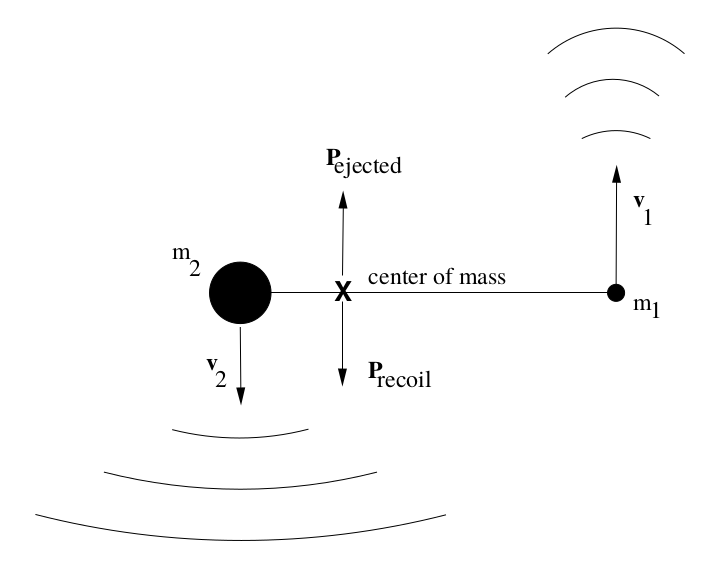
\includegraphics[width=0.6\linewidth]{Figures/binarySystem}
	\end{figure}
	
	Una forma de entender c\'omo sucede este fen\'omeno, es usando un sistema con masas desiguales. Se puede considerar dos cuerpos, uno con masa $m_1$ y otro con masa $m_2$, donde $m_2 > m_1$. En el caso cl\'asico, donde no existe ning\'un efecto nuevo, se tiene que el centro de masa orbitar\'ia alrededor de un c\'irculo. Sin embargo, cuando se tiene una onda que lleva energ\'ia y momento angular, se tiene que los cuerpos seguir\'ian una trayector\'ia en espiral, por lo cual al considerar toda una \'orbita ($\mathcal{O}$) se tendr\'ia que:
	\begin{equation}
		\int\limits_{\mathcal{O}_1} m_1\vec{v}_1dl \neq \int\limits_{\mathcal{O}_2} m_2\vec{v}_2dl 
	\end{equation}	
	
\section{Objetivo general}
%	Poner en funcionamiento el calorímetro 2277 Thermal Activity Monitor con el que se cuenta, en funcionamiento y adicionalmente calibrar el equipo para su uso en las investigaciones activas del grupo \groupname.
		
\section{Objetivos específicos}
%	\begin{itemize}
%		\item Ensamblar el equipo 2277 Thermal Activity Monitor.
%		\item Realizar el cableado y conexiones electrónicas pertinentes al mismo.
%		\item Calibración eléctrica, determinación de las señales de entrada y salida, flujo de las bombas hidráulicas y temperatura del baño.
%		\item Calibración química, determinación de la entalpía molar, energía libre de Gibbs, entropía, y constante de equilibrio, del acomplejamiento del catión bario con éter 18-corona-6.
%	\end{itemize}
%
%	\newpage

%\section{Justificación del proyecto}

%	
%	
%	
%	En general la calorimetría permite una gran variedad de análisis, muchos de ellos cuentan con aplicaciones industriales, comerciales, biológicas y químicas, permitiendo el entendimiento de las interacciones moleculares en soluciones \cite{blandamer1998titration}. Una ventaja de la calorimetría es que no es específica, ni invasiva además de no depender de las propiedades electroquímicas y ópticas de un sistema dado, siendo esto de vital importancia para las investigaciones de procesos biológicos, el estudio del crecimiento bacteriano y para la detección de compuestos biológicos \cite{winkelmann2004application}. Por otro lado la calorimetría también permite el estudio de la termodinámica en sistemas de absorción, bien sea por la universalidad de la absorción física en las superficies como catalizadores, o en procesos industriales como la separación de mezclas de gases \cite{morrison1987calorimetry}. Finalmente la calorimetría es el método clásico para la determinación de propiedades termodinámicas en las muestras, entre estas se encuentran la capacidad calorífica, la entalpía, entropía y energía libre de Gibbs, las cuales constituyen el punto de partida de gran cantidad de estudios teóricos, desarrollos y producción industrial de un compuesto químico \cite{wang2005determination, gaisford2016principles}.
%
%	El calorímetro 2277 Thermal Activity Monitor con el que cuenta el grupo de investigación se encuentra desarmado, a la espera de su ensamble y puesta en funcionamiento. Este instrumento permite monitorear una gran variedad de reacciones químicas y bioquímicas, lo anterior debido a su capacidad de cuantificar procesos exotérmicos y endotérmicos. Estas reacciones pueden ser estudiadas en el rango de 5 - 80 $^\circ$C \cite{Suurkuusk}. Este rango de temperaturas se debe al uso de un baño termostatado de 25 litros. Cuatro balones de medición independientes se encuentran sumergidos en este baño, permitiendo medidas con desviaciones de temperatura inferiores a $\pm2\times10^{-4}$ $^\circ$C, alcanzando de esta manera medidas en el rango de microvatios \cite{Suurkuusk}. Es por esta razón que poner en marcha y calibrar el equipo con el que cuenta el grupo de investigación resulta una contribución importante para el mismo, así como para el \deptname\ en general.
	
\section{Metodología}
	Las simulaciones ser\'an realizadas en el cluster de la universidad con el fin de paralelizar procesos, de forma que a haciendo uso de sus recursos se minimice el tiempo de simulación a fin de lograr la mayor cantidad de simulaciones posibles con el fin de obtener una cantidad significativa de datos de validación.
	
\section{Consideraciones éticas}
	Se manejará un repositorio de uso privado a través de Github en donde se encontrar\'an los códigos implementados en cada parte del proceso, junto con los resultados obtenidos, de forma que se asegure la reproducibilidad del modelo hallado, al mismo tiempo que se permita el seguimiento del uso de recursos. Adem\'as al mantener la informaci\'on abierta se asegura que no se están utilizando resultados obtenidos por otros investigadores de forma directa.
	
\section{Cronograma}
	\begin{table}[h]
		\centering
		\caption{Cronograma de actividades}
		\label{tb: cronograma}
		\footnotesize
		\begin{tabular}{|c|c|c|c|c|c|c|c|c|c|c|c|c|c|c|c|c|}
			\hline
			\rowcolor[HTML]{C0C0C0} 
			\cellcolor[HTML]{C0C0C0}                                       & \multicolumn{16}{c|}{\cellcolor[HTML]{C0C0C0}\textbf{Semana}} \\ \cline{2-17} 
			\rowcolor[HTML]{EFEFEF} 
			\multirow{-2}{*}{\cellcolor[HTML]{C0C0C0}\textbf{Actividades}} & \textbf{1} & \textbf{2} & \textbf{3} & \textbf{4} & \textbf{5} & \textbf{6} & \textbf{7} & \textbf{8} & \textbf{9} & \textbf{10} & \textbf{11} & \textbf{12} & \textbf{13} & \textbf{14} & \textbf{15} & \textbf{16} \\ \hline
			\cellcolor[HTML]{EFEFEF}
			\textbf{Revisión bibliográfica} & x & x & x & & & & x & x & x & x & & & & x & x & x \\ \hline
			\cellcolor[HTML]{EFEFEF}\textbf{Revisión de manuales} & x & x & x & x & & & & & & & & & & & & \\ \hline
			\cellcolor[HTML]{EFEFEF}\textbf{Ensamble del equipo} & x & x & x & x & & & & & & & & & & & & \\ \hline
			\cellcolor[HTML]{EFEFEF}\textbf{Cableado y electrónica} & & & x & x & x & x & & & & & & & & & & \\ \hline
			\cellcolor[HTML]{EFEFEF}\textbf{Calibración eléctrica} & & & & & & x & x & x & & & & & & & & \\ \hline
			\cellcolor[HTML]{EFEFEF}\textbf{Calibración química} & & & & & & & & & x & x & x & x & & & & \\ \hline
			\cellcolor[HTML]{EFEFEF}\textbf{Análisis de datos} & & & & & & & & & & & x & x & x & & & \\ \hline
			\cellcolor[HTML]{EFEFEF}\textbf{Elaboración del documento} & & & & & & & x & x & x & x & & & & x & x & x \\ \hline
			\cellcolor[HTML]{EFEFEF}\textbf{Presentación del proyecto} & & & & & & & & & & & & & & & & x \\ \hline
		\end{tabular}
	\end{table}
% !TeX spellcheck = en_US
% Chapter 1

%\chapter{Chapter Title Here} % Main chapter title
%
%\label{Chapter1} % For referencing the chapter elsewhere, use \ref{Chapter1} 

%----------------------------------------------------------------------------------------

% Define some commands to keep the formatting separated from the content
%\newcommand{\option}[1]{\texttt{\itshape#1}}

%----------------------------------------------------------------------------------------
\chapter{Spherical study}
			
	\section{Results}
	For a single simulation, the following data are saved: iteration time, current position, speed, and the black hole mass. With this information, accelerations and densities can be later reconstructed as on \autoref{fig: overallOutput}.
	\begin{figure}[h]
		\centering
		\includegraphics[width = 0.52\textwidth]{"../Files/Week 6/properties_s02v70"}
		\caption{Upper two plots show the output of a single simulation, while the lower one shows most the local properties per data point.}
		\label{fig: overallOutput}
	\end{figure}
	
	\subsection{Effect of the baryonic fraction}
	\begin{figure}[h]
		\centering
		\includegraphics[width = 0.7\textwidth]{"../Files/Week 5/baryonic_fraction_comparison"}
		\caption{.}
		\label{fig: baryonicfraction}
	\end{figure}
		
	\subsection{Effect of the power law exponent}
	\begin{figure}[h]
		\centering
		\begin{subfigure}[b]{0.49\textwidth}
			\includegraphics[width = \textwidth]{"../Files/Week 6/power_law"}
			\caption{.}
			\label{fig: powerLawOrbits}
		\end{subfigure}
		~ 
		\begin{subfigure}[b]{0.49\textwidth}
			\includegraphics[width=\textwidth]{"../Files/Week 6/power_law_density"}
			\caption{.}
			\label{fig: powerLawDensities}
		\end{subfigure}
		\caption{.}
		\label{fig: powerLaw}
	\end{figure}
	
	\subsection{Effect of the stellar fraction}
	\begin{figure}[h]
		\centering
		\includegraphics[width = 0.7\textwidth]{"../Files/Week 7/Symmetric/returntimes_stellar_speed"}
		\caption{.}
		\label{fig: stellarfraction}
	\end{figure} 
%\include{Chapters/Chapter3}
%\include{Chapters/Chapter4} 
%\include{Chapters/Chapter5} 

%----------------------------------------------------------------------------------------
%	THESIS CONTENT - APPENDICES
%----------------------------------------------------------------------------------------

%\appendix % Cue to tell LaTeX that the following "chapters" are Appendices

% Include the appendices of the thesis as separate files from the Appendices folder
% Uncomment the lines as you write the Appendices

%\include{Appendices/AppendixA}
%\include{Appendices/AppendixB}
%\include{Appendices/AppendixC}

%----------------------------------------------------------------------------------------
%	BIBLIOGRAPHY
%----------------------------------------------------------------------------------------

%\printbibliography[heading=bibintoc, title={Referencias}]

%----------------------------------------------------------------------------------------

\end{document}  
